%
% teil3.tex -- Beispiel-File für Teil 3
%
% (c) 2020 Prof Dr Andreas Müller, Hochschule Rapperswil
%
% !TEX root = ../../buch.tex
% !TEX encoding = UTF-8
%
\section{Kombination von Möbius Transformationen
\label{moebius:section:teil3}}
\kopfrechts{Kombination von Möbius-Transformationen}


Möbius-Transformationen können als Kombination einfacher Transformationen wie Translation, Skalierung und Inversion dargestellt werden.
\index{Skalierung}%

\begin{beispiel}
Als Beispiel für eine Möbius-Transformation betrachten wir die Abbildung
\[
f(z) = \frac{2z + 3}{z + 1}.
\]
Wir schreiben \( z \) in der Form
\[
z = x + i.
\]
Einsetzen ergibt
\[
f(z) = \frac{2(x + i) + 3}{(x + i) + 1},
\]
wobei wir zum Rechnen $z$ nehmen anstatt $x+i$.
Nun formen wir den Zähler um und erhalten
\[
f(z) = \frac{2(z + 1) + 1}{z + 1}.
\]
Durch das Aufteilen des Bruchs erhält man
\[
f(z) = \frac{2(z + 1)}{z + 1} + \frac{1}{z + 1}.
\]
Kürzen ergibt
\begin{equation}
	f(z) = 2 + \frac{1}{z + 1}.
\label{moebius:24.1}
\end{equation}
Die Formel
\eqref{moebius:24.1}
kann als Schrittweise zerlegung der Möbius Transformation interpretiert werden.
Der erste Schritt ist die Translation
\[
z_1 = z + 1.
\]
Dabei erfolgt eine Verschiebung der komplexen Ebene um \(1\) nach rechts.
Der zweite Schritt ist die Inversion
\[
z_2 = \frac{1}{z_1}.
\]
Punkte nahe beim Ursprung werden nach aussen abgebildet und umgekehrt.
Abschliessend erfolgt eine weitere Verschiebung um \(2\) nach rechts
\[
f(z) = 2 + z_2.
\]
Somit ergibt sich insgesamt die Transformation von Formel \eqref{moebius:24.1}.
\begin{figure}
	\centering
	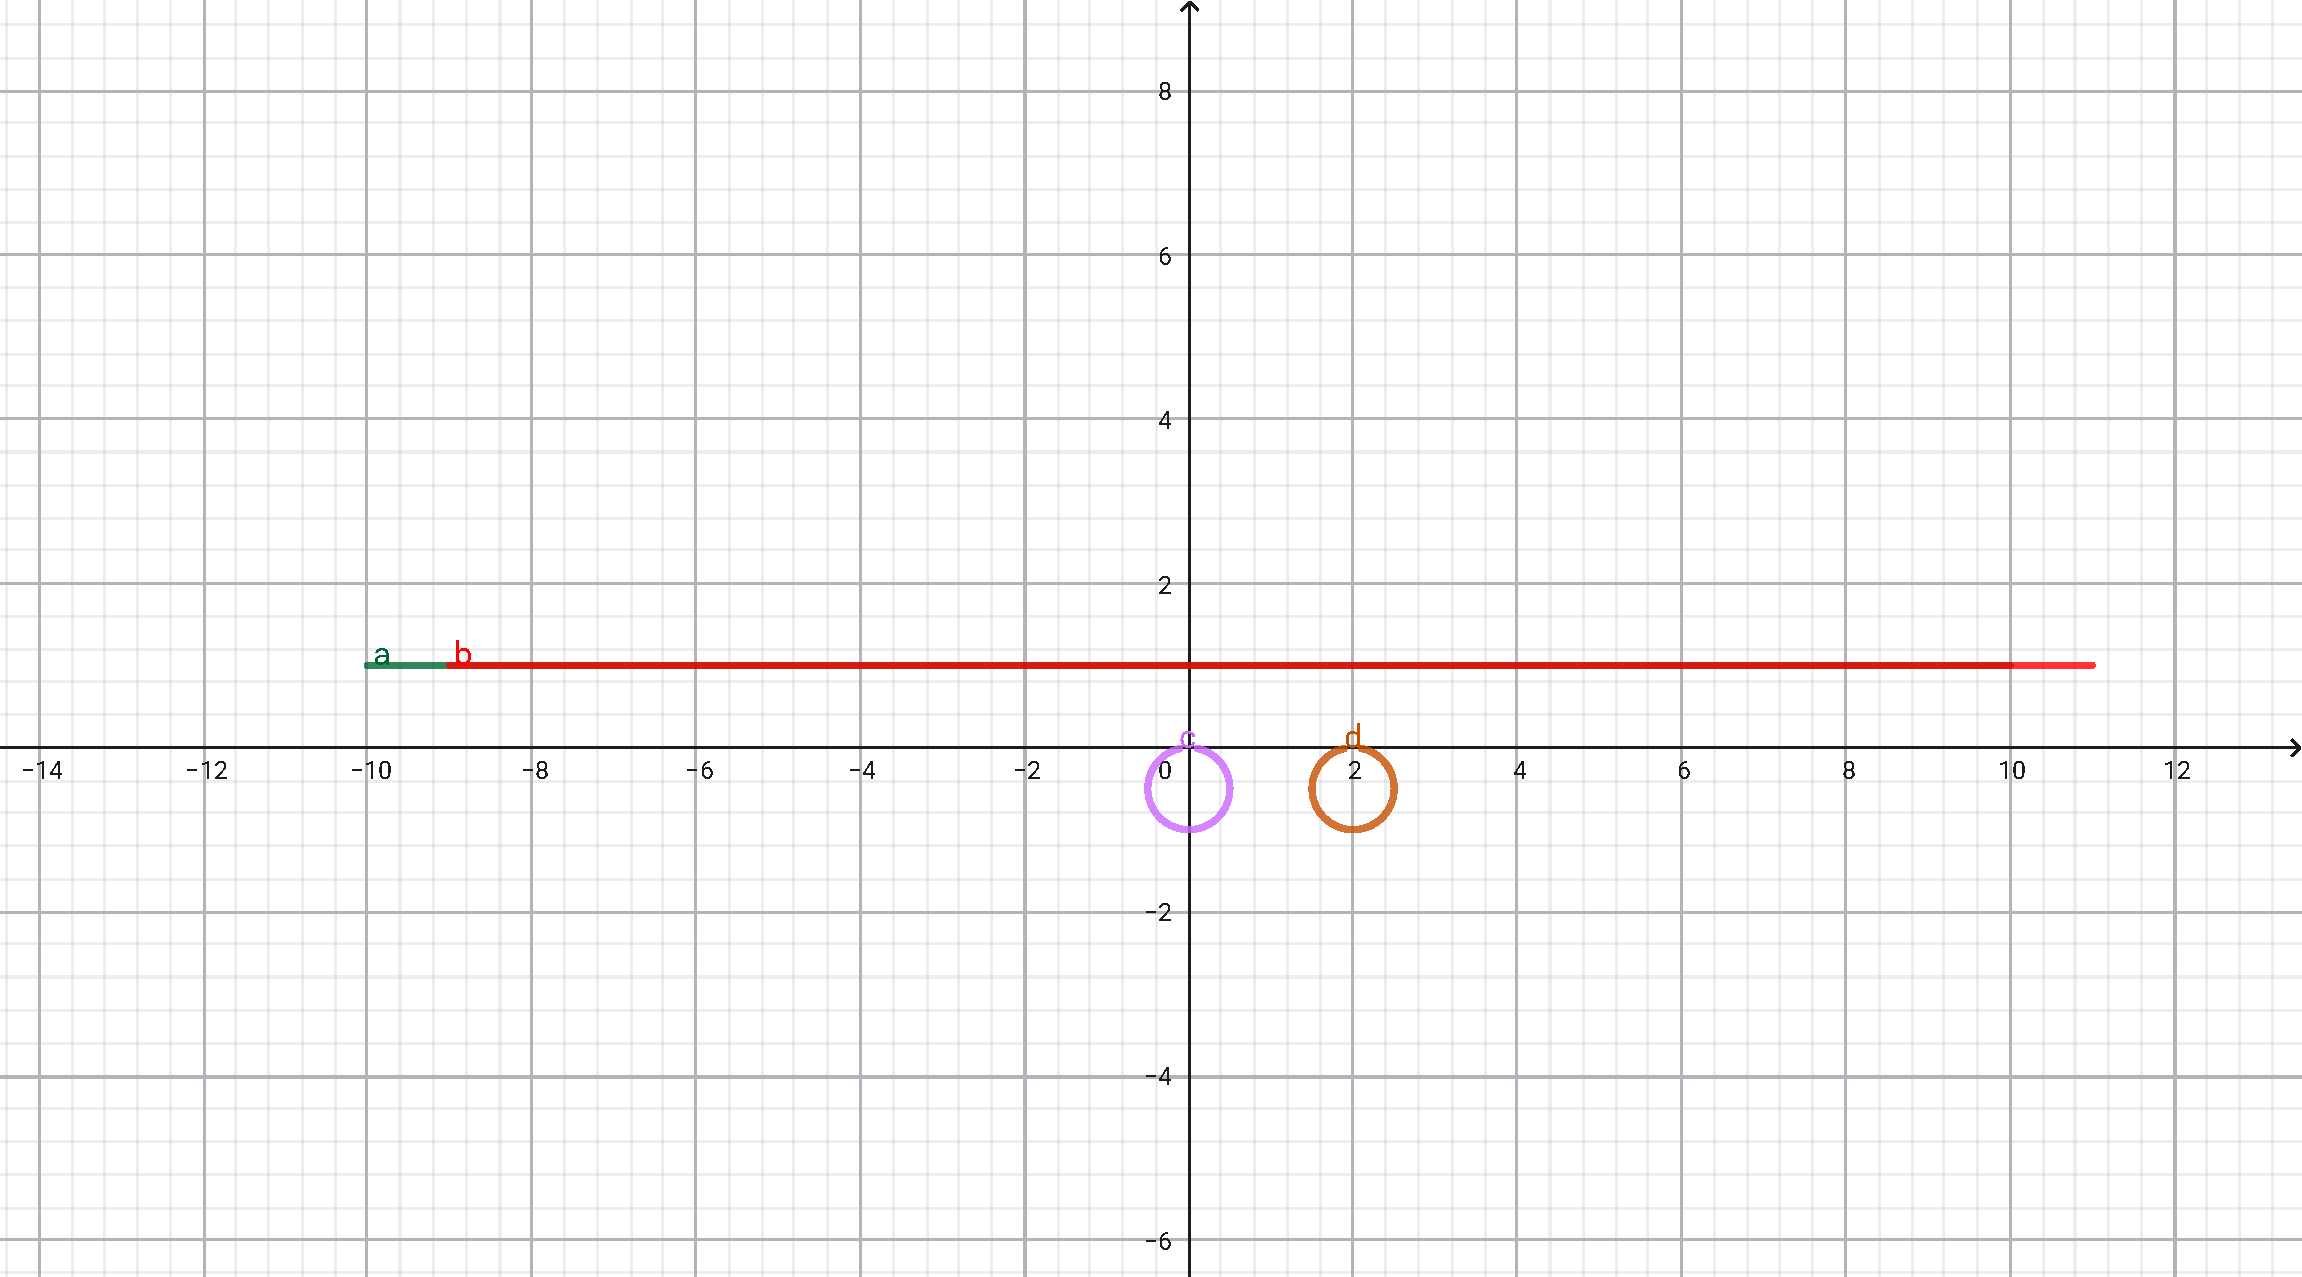
\includegraphics[width=1\textwidth]{papers/moebius/bild6.pdf}
	\caption{Kombination der Translationen (erstellt mit GeoGebra)
	\label{moebius:24.6}}
\end{figure} 
In der Abbildung \ref{moebius:24.6} sieht man gut, wie (a) unsere
Startgerade ist, bei (b) die Verschiebung um 1, bei (c) die Inversion
von der Gerade zum Kreis, weil die Gerade nicht durch den Nullpunkt
geht und bei (d) nochmals eine Verschiebung um 2 stattfindet.
\end{beispiel}
